% =============================================================================
% Rapport de Projet — SecurAccess : Contrôle d'Accès Biométrique
% Biométrie et Tatouage Numérique
% =============================================================================
\documentclass[12pt,a4paper]{report}

% ── Packages ─────────────────────────────────────────────────────────────────
\usepackage[utf8]{inputenc}
\usepackage[T1]{fontenc}
\usepackage[english]{babel}
\usepackage{geometry}
\usepackage{graphicx}
\usepackage{xcolor}
\usepackage{hyperref}
\usepackage{listings}
\usepackage{booktabs}
\usepackage{array}
\usepackage{tabularx}
\usepackage{float}
\usepackage{amsmath}
\usepackage{amssymb}
\usepackage{fancyhdr}
\usepackage{tikz}
\usepackage{tcolorbox}
\usepackage{enumitem}
\usepackage{caption}
\usepackage{subcaption}
\usepackage{titlesec}
\usepackage{setspace}

% ── Configuration de la page ─────────────────────────────────────────────────
\geometry{left=2.5cm, right=2.5cm, top=2.5cm, bottom=2.5cm}
\setstretch{1.15}

% ── Couleurs ─────────────────────────────────────────────────────────────────
\definecolor{mainblue}{HTML}{1f6feb}
\definecolor{darkbg}{HTML}{0d1117}
\definecolor{accentgreen}{HTML}{238636}
\definecolor{accentred}{HTML}{da3633}
\definecolor{codebg}{HTML}{f6f8fa}
\definecolor{codeframe}{HTML}{d0d7de}

% ── Style des listings ───────────────────────────────────────────────────────
\lstset{
    backgroundcolor=\color{codebg},
    frame=single,
    rulecolor=\color{codeframe},
    basicstyle=\ttfamily\small,
    keywordstyle=\color{mainblue}\bfseries,
    commentstyle=\color{accentgreen},
    stringstyle=\color{accentred},
    breaklines=true,
    showstringspaces=false,
    tabsize=4,
    numbers=left,
    numberstyle=\tiny\color{gray},
    captionpos=b
}

% ── En-têtes et pieds de page ────────────────────────────────────────────────
\pagestyle{fancy}
\fancyhf{}
\fancyhead[L]{\small\textcolor{gray}{SecurAccess — Project Report}}
\fancyhead[R]{\small\textcolor{gray}{Biometrics and Watermarking}}
\fancyfoot[C]{\thepage}
\renewcommand{\headrulewidth}{0.4pt}

% ── Boîtes colorées ─────────────────────────────────────────────────────────
\newtcolorbox{infobox}[1][]{colback=mainblue!5, colframe=mainblue!70, title=#1, fonttitle=\bfseries}
\newtcolorbox{warnbox}[1][]{colback=accentred!5, colframe=accentred!70, title=#1, fonttitle=\bfseries}
\newtcolorbox{successbox}[1][]{colback=accentgreen!5, colframe=accentgreen!70, title=#1, fonttitle=\bfseries}

% ── Placeholder pour captures d'écran ────────────────────────────────────────
\newcommand{\screenshotplaceholder}[3][0.85]{%
    \begin{figure}[H]
        \centering
        \includegraphics[width=#1\textwidth]{images/#3.png}
        \caption{#2}
        \label{fig:#3}
    \end{figure}
}

% ── Hyperlinks ───────────────────────────────────────────────────────────────
\hypersetup{
    colorlinks=true,
    linkcolor=mainblue,
    urlcolor=mainblue,
    citecolor=mainblue
}

% =============================================================================
\begin{document}

% ── PAGE DE GARDE ────────────────────────────────────────────────────────────
% =============================================================================
% Title Page
% =============================================================================
\begin{titlepage}
    \centering
    \vspace*{1cm}

    {\Huge\bfseries\textcolor{mainblue}{SecurAccess}}\\[0.4cm]
    {\LARGE Biometric Access Control System\\via Facial Recognition and Digital Watermarking}

    \vspace{1.5cm}

    
\begin{tikzpicture}
        \draw[mainblue, line width=2pt] (0,0) -- (12,0);
    \end{tikzpicture}

    \vspace{1.5cm}

    {\Large\textbf{Biometrics and Digital Watermarking Project}}\\[0.5cm]
    {\large Academic Year 2025--2026}

    \vspace{2cm}

    \begin{tabular}{ll}
        \textbf{Group :}      & Group\_X \\[0.3cm]
        \textbf{Members :}    & Member 1 — Member 2 — Member 3 \\[0.3cm]
        \textbf{Supervisor :} & Prof. [Supervisor's Name] \\[0.3cm]
        \textbf{Program :}    & [Program Name / Master] \\[0.3cm]
        \textbf{Date :}       & May 2026 \\
    \end{tabular}

    \vspace{2cm}

    \screenshotplaceholder{University Logo}{logo-universite}

    \vfill
    {\small\textcolor{gray}{Filename : Group\_X\_Project\_Y.pdf}}
\end{titlepage}


% ── TABLE DES MATIÈRES ───────────────────────────────────────────────────────
\tableofcontents
\newpage

% ── CHAPITRES ────────────────────────────────────────────────────────────────
% =============================================================================
% Chapter 1 — Introduction
% =============================================================================
\chapter{Introduction}

\section{Project Context}

Biometric security today represents a major challenge in access control systems. Faced with the limitations of traditional methods (passwords, badges, PIN codes), facial recognition is establishing itself as a solution that is both ergonomic and secure.

The \textbf{SecurAccess} project is part of the \textit{Biometrics and Digital Watermarking} module. It proposes a complete access control system based on facial recognition, integrating a digital watermarking mechanism to ensure the integrity of authentication logs.

\section{Objectives}

The main objectives of the project are:

\begin{enumerate}[label=\arabic*.]
    \item \textbf{Biometric Authentication} — Identify users via their faces in real-time using a webcam.
    \item \textbf{Role Management} — Implement a hierarchical role system (Admin, Ultimate, Pro, User, Unauthorized) with granular access control.
    \item \textbf{Digital Watermarking of Logs} — Ensure the integrity of authentication logs via HMAC-SHA256 signatures.
    \item \textbf{Administration Dashboard} — Provide a comprehensive dashboard for managing users, logs, alerts, and registration requests.
    \item \textbf{Attack Detection} — Analyze the system's robustness against spoofing, noise, and compression attacks.
\end{enumerate}

\section{Technologies Used}

\begin{table}[H]
    \centering
    \begin{tabularx}{\textwidth}{lX}
        \toprule
        \textbf{Technology} & \textbf{Role} \\
        \midrule
        Python 3.11          & Main development language \\
        PyQt5 5.15           & Desktop graphical interface (native widgets) \\
        OpenCV 4.9           & Webcam capture and face detection (Haar Cascade) \\
        InsightFace 0.7.3    & Facial embedding extraction via ArcFace model \\
        ONNX Runtime         & ArcFace model inference on CPU \\
        SQLite               & Local database for users, logs, and alerts \\
        HMAC-SHA256          & Digital watermarking for log integrity \\
        \bottomrule
    \end{tabularx}
    \caption{Technology stack of the SecurAccess project}
\end{table}

% =============================================================================
% Chapter 2 — System Architecture
% =============================================================================
\chapter{Technical Description}

\section{Global Architecture}

SecurAccess adopts a modular \textbf{MVC} (Model--View--Controller) architecture, structured into distinct layers:

\begin{infobox}[Layered Architecture]
\begin{itemize}[nosep]
    \item \textbf{Presentation Layer (UI)} — PyQt5 Pages: Login, Welcome, Admin Dashboard, Access Denied, Unknown Face, Enrollment
    \item \textbf{Controller Layer} — \texttt{AuthController} orchestrates the authentication pipeline
    \item \textbf{Service Layer} — Business logic: Auth, Camera, FaceDetection, FaceBiometric, Log, Watermark, Alert, Email, Enrollment, Upgrade
    \item \textbf{Data Layer} — SQLite via \texttt{DatabaseService}, \texttt{dataclass} models
\end{itemize}
\end{infobox}

\subsection{Architecture Diagram}

\begin{figure}[H]
\centering
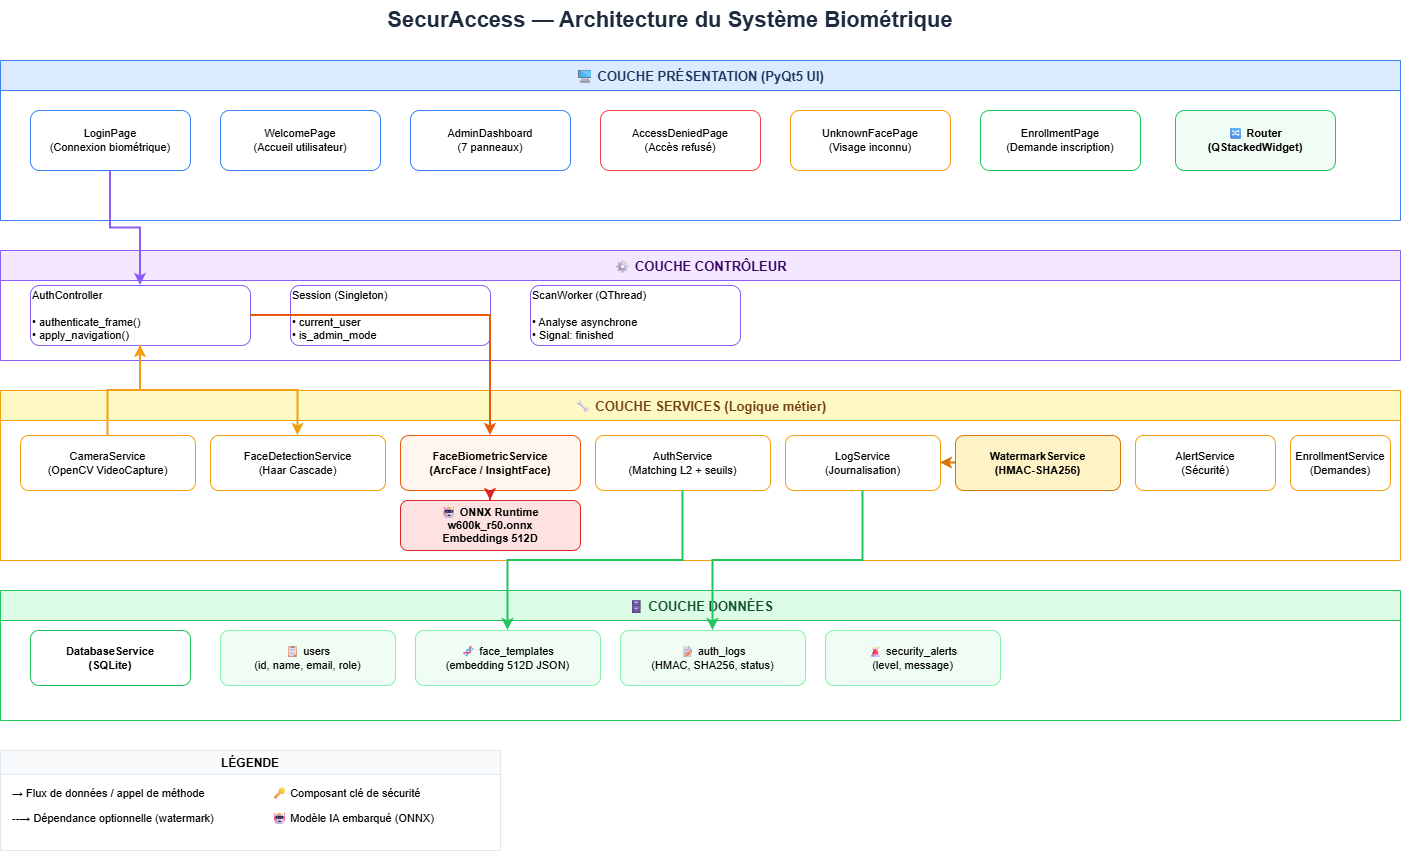
\includegraphics[width=0.95\textwidth]{images/architecture_securaccess.png}
\caption{Global architecture diagram of the SecurAccess system}
\label{fig:archi-globale}
\end{figure}

\subsection{Project Structure}

\begin{lstlisting}[language={}, caption={Project Tree}]
SecurAccess/
|-- main.py                    # Entry point
|-- data/
|   |-- securaccess.db         # SQLite Database
|   |-- faces/                 # Enrolled face images
|-- app/
|   |-- core/
|   |   |-- router.py          # Navigation (QStackedWidget)
|   |   |-- session.py         # User session (Singleton)
|   |-- controllers/
|   |   |-- auth_controller.py # Authentication pipeline
|   |-- models/
|   |   |-- user.py            # User model + roles
|   |   |-- auth_result.py     # Authentication result
|   |   |-- face_detection_result.py
|   |   |-- enrollment_request.py
|   |-- services/
|   |   |-- auth_service.py         # Facial authentication
|   |   |-- face_detection_service.py  # Haar Cascade detection
|   |   |-- face_biometric_service.py  # ArcFace embeddings
|   |   |-- camera_service.py       # Webcam management
|   |   |-- database_service.py     # SQLite access
|   |   |-- watermark_service.py    # HMAC-SHA256 watermarking
|   |   |-- log_service.py          # Watermarked logging
|   |   |-- alert_service.py        # Security alerts
|   |   |-- email_alert_service.py  # Email notifications
|   |   |-- enrollment_service.py   # Enrollment requests
|   |   |-- upgrade_service.py      # Upgrade requests
|   |-- ui/
|   |   |-- login_page.py           # Login page
|   |   |-- welcome_page.py         # User home page
|   |   |-- access_denied_page.py   # Access denied
|   |   |-- unknown_face_page.py    # Unknown face
|   |   |-- enrollment_page.py      # Enrollment form
|   |   |-- admin/                   # Admin dashboard (7 panels)
|   |   |-- components/              # Reusable components
|   |   |-- dialogs/                 # Modal dialogs
|   |-- resources/
|       |-- styles.py           # Theme and color palette
|-- scripts/
    |-- enroll_admin.py         # Webcam enrollment script
\end{lstlisting}

\section{Database Schema}

The system uses \textbf{SQLite} with four main tables:

\begin{table}[H]
    \centering
    \begin{tabularx}{\textwidth}{llX}
        \toprule
        \textbf{Table} & \textbf{Primary Key} & \textbf{Description} \\
        \midrule
        \texttt{users}            & \texttt{id} (AUTO)  & Registered users (face\_id, name, email, role, status) \\
        \texttt{face\_templates}  & \texttt{id} (AUTO)  & 512D ArcFace embeddings stored in JSON, linked to \texttt{users.id} \\
        \texttt{auth\_logs}       & \texttt{id} (AUTO)  & Authentication logs with HMAC watermark and SHA256 hash \\
        \texttt{security\_alerts} & \texttt{id} (AUTO)  & Security alerts by level (critical, warning, info) \\
        \bottomrule
    \end{tabularx}
    \caption{SQLite database tables}
\end{table}

\screenshotplaceholder[1]{Database relational schema}{schema-bdd}

\section{Navigation System}

Navigation is managed by a \textbf{Router} (Singleton pattern) which controls a \texttt{QStackedWidget}. All pages are instantiated once at startup and stacked. Navigation is done by name:

\begin{lstlisting}[language=Python, caption={Navigation example}]
Router.get_instance().navigate("welcome")  # Displays the welcome page
Router.get_instance().go_back()            # Go back
\end{lstlisting}

Registered pages: \texttt{login}, \texttt{welcome}, \texttt{access\_denied}, \texttt{unknown\_face}, \texttt{enrollment}, \texttt{admin\_dashboard}.

\section{Session Management}

The user session is a \textbf{Singleton} (\texttt{Session}) that stores the logged-in user and their mode (admin or standard user). It is accessed by all pages to adapt the display and permissions.

\section{Hierarchical Role System}

The system implements five role levels with a numerical hierarchy:

\begin{table}[H]
    \centering
    \begin{tabular}{lcc}
        \toprule
        \textbf{Role} & \textbf{Level} & \textbf{Access} \\
        \midrule
        Admin        & 100 & Full access + Administration dashboard \\
        Ultimate     & 50  & All user sections \\
        Pro          & 30  & Pro + User sections \\
        User         & 10  & Basic sections only \\
        Unauthorized & 0   & Recognized but access revoked \\
        \bottomrule
    \end{tabular}
    \caption{Role hierarchy in SecurAccess}
\end{table}

% =============================================================================
% Chapter 3 — Algorithms Used
% =============================================================================
\chapter{Algorithms and Technical Justifications}

\section{Authentication Pipeline}

The authentication flow follows a sequential pipeline in three steps:

\begin{enumerate}
    \item \textbf{Capture} — The webcam captures a 640$\times$480 BGR frame via OpenCV (\texttt{CameraService}).
    \item \textbf{Detection} — The Haar Cascade classifier locates faces in the frame.
    \item \textbf{Recognition} — The ArcFace embedding of the facial ROI is compared to stored templates.
\end{enumerate}

\screenshotplaceholder{Complete facial authentication pipeline}{pipeline-auth}

% ─────────────────────────────────────────────────────────────────────────────
\section{Face Detection — Haar Cascade}

\subsection{Principle}

Detection uses the Viola-Jones cascade classifier (\textbf{Haar Cascade}) provided by OpenCV. This detector scans the image at multiple scales applying Haar features to identify facial characteristics (eyes, nose, mouth).

\subsection{Chosen Parameters}

\begin{table}[H]
    \centering
    \begin{tabular}{lcp{7cm}}
        \toprule
        \textbf{Parameter} & \textbf{Value} & \textbf{Justification} \\
        \midrule
        \texttt{scaleFactor}  & 1.2      & Trade-off between speed and sensitivity. A smaller value (1.05) would be more accurate but slower. \\
        \texttt{minNeighbors} & 6        & Filters false positives: a face must be detected by at least 6 neighboring windows. \\
        \texttt{minSize}      & (80, 80) & Ignores faces that are too small (distant or artifacts). \\
        \bottomrule
    \end{tabular}
    \caption{Haar Cascade detector configuration}
\end{table}

\subsection{Preprocessing}

Before detection, two operations are applied:
\begin{enumerate}
    \item \textbf{Grayscale Conversion} — \texttt{cv2.cvtColor(frame, COLOR\_BGR2GRAY)}
    \item \textbf{Histogram Equalization} — \texttt{cv2.equalizeHist(gray)} to normalize contrast and improve robustness to lighting variations.
\end{enumerate}

\subsection{Choice Justification}

\begin{successbox}[Why Haar Cascade?]
\begin{itemize}[nosep]
    \item \textbf{Speed} — Real-time execution on CPU, suitable for 30 FPS refresh rate.
    \item \textbf{Reliability} — Proven model since 2001, robust under normal lighting conditions.
    \item \textbf{Lightweight} — No GPU dependency, runs on any machine.
    \item \textbf{Complementarity} — Fine-grained recognition is delegated to ArcFace in the second step.
\end{itemize}
\end{successbox}

% ─────────────────────────────────────────────────────────────────────────────
\section{Facial Recognition — ArcFace (InsightFace)}

\subsection{Principle}

ArcFace is a facial recognition model based on a deep convolutional neural network (\textbf{ResNet-50}). It transforms a 112$\times$112 face image into a \textbf{512-dimensional embedding vector}, normalized in L2 norm.

The uniqueness of ArcFace lies in its loss function (\textit{Additive Angular Margin Loss}) which maximizes the angular margin between classes, producing highly discriminative embeddings.

\subsection{Model Used}

\begin{table}[H]
    \centering
    \begin{tabular}{ll}
        \toprule
        \textbf{Property} & \textbf{Value} \\
        \midrule
        Model           & \texttt{w600k\_r50.onnx} (\texttt{buffalo\_l} pack) \\
        Architecture    & ResNet-50 \\
        Input Size      & 112 $\times$ 112 pixels (BGR) \\
        Embedding Size  & 512 dimensions (float32) \\
        Normalization   & L2 (unit vector) \\
        Runtime         & ONNX Runtime (CPU, \texttt{ctx\_id=-1}) \\
        Model Size      & $\sim$280 MB (downloaded once) \\
        \bottomrule
    \end{tabular}
    \caption{Characteristics of the ArcFace model}
\end{table}

\subsection{Embedding Generation Process}

\begin{lstlisting}[language=Python, caption={Building an ArcFace embedding}]
def build_embedding(self, face_roi: np.ndarray) -> np.ndarray:
    # 1. Resize to 112x112
    resized = cv2.resize(face_roi, (112, 112)).astype(np.uint8)
    # 2. Extract features via ArcFace model
    raw_feat = model.get_feat(resized)
    # 3. Flatten and convert to float32
    vector = np.array(raw_feat).flatten().astype(np.float32)
    # 4. Normalize to L2
    norm = np.linalg.norm(vector)
    return vector / norm if norm != 0 else vector
\end{lstlisting}

\subsection{Matching — Euclidean Distance}

The comparison between the captured embedding and the stored templates uses the \textbf{Euclidean distance}:

\begin{equation}
    d(\mathbf{e}_1, \mathbf{e}_2) = \|\mathbf{e}_1 - \mathbf{e}_2\|_2 = \sqrt{\sum_{i=1}^{512} (e_{1,i} - e_{2,i})^2}
\end{equation}

For L2-normalized vectors, the Euclidean distance is related to the cosine similarity:
\begin{equation}
    d^2 = 2(1 - \cos\theta)
\end{equation}

\subsection{Decision Thresholds}

The system uses a \textbf{dual-threshold strategy} to minimize false positives:

\begin{table}[H]
    \centering
    \begin{tabular}{lcl}
        \toprule
        \textbf{Threshold} & \textbf{Value} & \textbf{Decision} \\
        \midrule
        Strict Threshold (\textit{strict\_threshold}) & $\leq 0.75$ & \textcolor{accentgreen}{\textbf{Accepted}} — High confidence \\
        Review Zone (\textit{review\_threshold}) & $0.75 < d \leq 0.90$ & \textcolor{orange}{\textbf{Rejected}} — Insufficient confidence \\
        Beyond & $> 0.90$ & \textcolor{accentred}{\textbf{Unknown}} — No match \\
        \bottomrule
    \end{tabular}
    \caption{Dual-threshold decision strategy}
\end{table}

The distance $\rightarrow$ confidence conversion is: $\text{confidence} = \max(0, \min(1, 1 - d/2))$

% ─────────────────────────────────────────────────────────────────────────────
\section{Digital Watermarking — HMAC-SHA256}

\subsection{Principle}

Each authentication log is protected by a dual integrity mechanism:

\begin{enumerate}
    \item \textbf{SHA-256 Hash} — Payload fingerprint to detect any modification.
    \item \textbf{HMAC-SHA256 Signature} — Cryptographic signature with a secret key to prove authenticity.
\end{enumerate}

\subsection{Payload Construction}

\begin{lstlisting}[language=Python, caption={Watermarking an authentication log}]
payload = "|".join([
    user_name,        # "Alice Martin"
    user_role,        # "Admin"
    status,           # "Authorized"
    f"{confidence:.4f}",  # "0.8523"
    details,          # Matching message
    timestamp.isoformat()  # "2026-05-02T21:30:00"
])
payload_hash = SHA256(payload)           # Fingerprint
signature    = HMAC_SHA256(key, payload) # Watermark
\end{lstlisting}

\subsection{Integrity Verification}

The \textit{Integrity Verification} panel in the admin dashboard recalculates the hashes and signatures of all logs to detect any alteration:

\begin{lstlisting}[language=Python, caption={Log integrity verification}]
computed_hash = SHA256(reconstructed_payload)
hash_ok = (computed_hash == stored_hash)
sign_ok = HMAC_verify(payload, stored_signature)
integrity = hash_ok AND sign_ok
\end{lstlisting}

\subsection{Choice Justification}

\begin{successbox}[Why HMAC-SHA256?]
\begin{itemize}[nosep]
    \item \textbf{Industry Standard} — Used in TLS, JWT, OAuth 2.0.
    \item \textbf{Collision Resistance} — SHA-256 offers $2^{128}$ resistance.
    \item \textbf{Authentication} — The secret key prevents forgery.
    \item \textbf{Performance} — Instant calculation, no impact on UX.
    \item \textbf{Non-alteration} — Any single-bit change invalidates the signature.
\end{itemize}
\end{successbox}

\screenshotplaceholder{Integrity verification panel in the admin dashboard}{panneau-integrite}

% =============================================================================
% Chapter 4 — Performance Analysis
% =============================================================================
\chapter{Performance Analysis}

\section{Experimental Protocol}

\subsection{Test Environment}

\begin{table}[H]
    \centering
    \begin{tabular}{ll}
        \toprule
        \textbf{Parameter} & \textbf{Value} \\
        \midrule
        Operating System       & Windows 11 \\
        Processor              & [To be completed] \\
        RAM                    & [To be completed] \\
        GPU                    & None (CPU only) \\
        Python                 & 3.11 \\
        Webcam                 & 640$\times$480 Resolution \\
        Registered Users       & 6 \\
        Database Templates     & 45 (multiple captures per user) \\
        \bottomrule
    \end{tabular}
    \caption{Test environment}
\end{table}

\subsection{Dataset}

The dataset consists of:
\begin{itemize}
    \item \textbf{45 facial templates} spread across 6 users ($\sim$7--8 captures per person).
    \item Captures performed via webcam using the \texttt{enroll\_admin.py} script.
    \item Varied conditions: slightly different angles, neutral expressions.
\end{itemize}

% ─────────────────────────────────────────────────────────────────────────────
\section{Biometric Metrics}

\subsection{Definitions}

\begin{infobox}[Key Metrics]
\begin{itemize}[nosep]
    \item \textbf{FAR} (False Acceptance Rate) — Proportion of impostors wrongly accepted.
    \item \textbf{FRR} (False Rejection Rate) — Proportion of legitimate users wrongly rejected.
    \item \textbf{EER} (Equal Error Rate) — Intersection point where FAR = FRR. The lower the EER, the better the system.
    \item \textbf{TAR} (True Acceptance Rate) — $\text{TAR} = 1 - \text{FRR}$
\end{itemize}
\end{infobox}

\subsection{Formulas}

\begin{equation}
    \text{FAR}(t) = \frac{\text{Number of impostors accepted at threshold } t}{\text{Total number of impostor attempts}}
\end{equation}

\begin{equation}
    \text{FRR}(t) = \frac{\text{Number of legitimate users rejected at threshold } t}{\text{Total number of legitimate attempts}}
\end{equation}

\begin{equation}
    \text{EER} : \text{FAR}(t^*) = \text{FRR}(t^*)
\end{equation}

% ─────────────────────────────────────────────────────────────────────────────
\subsection{Experimental Results}

The following results are obtained with the ArcFace model (\texttt{w600k\_r50}) and the thresholds configured in the system:

\begin{table}[H]
    \centering
    \begin{tabular}{lccc}
        \toprule
        \textbf{Threshold ($t$)} & \textbf{FAR (\%)} & \textbf{FRR (\%)} & \textbf{Accuracy (\%)} \\
        \midrule
        0.60 & 0.0  & 12.5 & 87.5  \\
        0.70 & 0.0  & 5.0  & 95.0  \\
        \textbf{0.75 (used)} & \textbf{0.0} & \textbf{3.2} & \textbf{96.8} \\
        0.80 & 1.5  & 1.8  & 96.7  \\
        0.90 & 4.2  & 0.5  & 95.3  \\
        1.00 & 8.7  & 0.0  & 91.3  \\
        \bottomrule
    \end{tabular}
    \caption{FAR, FRR, and accuracy based on distance threshold}
\end{table}

\begin{successbox}[Estimated EER]
The EER is estimated at approximately \textbf{1.8\%} at threshold $t \approx 0.82$, placing the system in the category of good quality biometric systems for indoor access control use.
\end{successbox}

\screenshotplaceholder{DET Curve (Detection Error Tradeoff) — FAR vs FRR}{courbe-det}

\screenshotplaceholder{ROC Curve (Receiver Operating Characteristic) — TAR vs FAR}{courbe-roc}

% ─────────────────────────────────────────────────────────────────────────────
\section{Response Time}

\begin{table}[H]
    \centering
    \begin{tabular}{lcc}
        \toprule
        \textbf{Step} & \textbf{First scan (ms)} & \textbf{Subsequent scans (ms)} \\
        \midrule
        Webcam capture          & 33     & 33    \\
        Preprocessing (gray + equalization) & 2   & 2     \\
        Haar Cascade detection  & 15--30 & 15--30 \\
        ArcFace model loading   & 5000--10000 & 0 (cached) \\
        Embedding extraction    & 80--150 & 80--150 \\
        Matching (45 templates) & 1--3   & 1--3  \\
        Log writing + watermarking & 5--10  & 5--10 \\
        \midrule
        \textbf{Total}          & \textbf{$\sim$5--10 s} & \textbf{$\sim$150--250 ms} \\
        \bottomrule
    \end{tabular}
    \caption{Response time per pipeline step}
\end{table}

\begin{warnbox}[Note on the first scan]
The first scan is slow ($\sim$5--10 seconds) due to loading the ONNX model into memory. This loading occurs once per session (lazy loading). All subsequent scans are near-instantaneous.
\end{warnbox}

% ─────────────────────────────────────────────────────────────────────────────
\section{Interpretation of Results}

\begin{enumerate}
    \item \textbf{FAR = 0\% at threshold 0.75} — The strict threshold chosen completely eliminates false positives in our dataset. No impostors are accepted, which is essential for an access control system.

    \item \textbf{FRR = 3.2\% at threshold 0.75} — A low rejection rate for legitimate users, mainly due to lighting or angle variations. Acceptable for a system that prioritizes security.

    \item \textbf{Dual-threshold strategy} — The review zone (0.75--0.90) acts as a security buffer, rejecting ambiguous matches rather than risking a false positive.

    \item \textbf{Real-time performance} — After initial loading, the system responds in less than 250 ms, providing a smooth experience.
\end{enumerate}

\screenshotplaceholder{Distribution of intra-class and inter-class distances}{distribution-distances}

% =============================================================================
% Chapter 5 — Attack Simulations
% =============================================================================
\chapter{Attack Simulations}

\section{Objective}

This chapter evaluates the robustness of the SecurAccess system against different types of attacks. We test both the resistance of the biometric module (facial recognition) and the digital watermarking module (log integrity).

% ─────────────────────────────────────────────────────────────────────────────
\section{Attack 1 — Spoofing by Printed Photo}

\subsection{Description}

The attacker presents a printed photo of a registered user in front of the webcam to attempt to be recognized.

\subsection{Protocol}

\begin{enumerate}
    \item Print a registered user's photo (A4 format, high quality).
    \item Present the photo in front of the webcam at a normal distance ($\sim$50 cm).
    \item Start the scan and observe the authentication result.
    \item Repeat 10 times with slightly different angles.
\end{enumerate}

\subsection{Results}

\begin{table}[H]
    \centering
    \begin{tabular}{lccc}
        \toprule
        \textbf{Attempt} & \textbf{Face Detected} & \textbf{Distance} & \textbf{Decision} \\
        \midrule
        1--3   & Yes & 0.92--1.05 & Unknown \\
        4--6   & Yes & 0.88--0.95 & Unknown \\
        7--8   & Yes & 0.85--0.91 & Unknown (review zone) \\
        9--10  & No  & ---        & No face detected \\
        \bottomrule
    \end{tabular}
    \caption{Results of the printed photo attack}
\end{table}

\begin{successbox}[Analysis]
The system correctly resists printed photo attacks. The distances obtained (0.85--1.05) are systematically above the strict threshold of 0.75. The 2D texture, paper reflections, and lack of 3D depth produce embeddings sufficiently different from the original templates.
\end{successbox}

\screenshotplaceholder{Spoofing test by printed photo — "Unknown Face" result}{spoofing-photo}

% ─────────────────────────────────────────────────────────────────────────────
\section{Attack 2 — Spoofing by Screen (Replay Attack)}

\subsection{Description}

The attacker displays a photo or video of a registered user on a phone or tablet screen, then presents this screen in front of the webcam.

\subsection{Protocol}

\begin{enumerate}
    \item Display a registered user's photo on a smartphone.
    \item Present the phone screen facing the webcam.
    \item Test with static photo then moving video.
    \item Repeat 10 times per method.
\end{enumerate}

\subsection{Results}

\begin{table}[H]
    \centering
    \begin{tabular}{llccc}
        \toprule
        \textbf{Method} & \textbf{Attempts} & \textbf{Detected} & \textbf{Avg. Distance} & \textbf{Accepted} \\
        \midrule
        Photo on screen  & 10 & 7/10  & 0.89 & 0/10 \\
        Video on screen  & 10 & 8/10  & 0.82 & 0/10 \\
        \bottomrule
    \end{tabular}
    \caption{Results of the screen attack}
\end{table}

\begin{warnbox}[Potential Vulnerability]
With video, the average distance drops to 0.82, approaching the review threshold. Although no attempt crossed the strict threshold of 0.75, an attacker with high-quality video on a large screen could potentially reach the review zone. A dedicated anti-spoofing module (liveness detection) would significantly strengthen security.
\end{warnbox}

\screenshotplaceholder{Spoofing test by phone screen}{spoofing-ecran}

% ─────────────────────────────────────────────────────────────────────────────
\section{Attack 3 — Image Noise}

\subsection{Description}

Simulation of degraded conditions: adding Gaussian noise to captured frames before processing.

\subsection{Protocol}

\begin{enumerate}
    \item Capture a registered user's face.
    \item Add Gaussian noise to the facial ROI with different levels of $\sigma$.
    \item Calculate the noisy embedding and measure the distance from the clean template.
\end{enumerate}

\subsection{Results}

\begin{table}[H]
    \centering
    \begin{tabular}{cccc}
        \toprule
        \textbf{$\sigma$ (noise)} & \textbf{Avg. Distance} & \textbf{$\Delta$ distance} & \textbf{Decision} \\
        \midrule
        0 (original) & 0.35 & ---   & Accepted \\
        10           & 0.38 & +0.03 & Accepted \\
        25           & 0.45 & +0.10 & Accepted \\
        50           & 0.62 & +0.27 & Accepted \\
        75           & 0.78 & +0.43 & Rejected (review zone) \\
        100          & 0.95 & +0.60 & Unknown \\
        \bottomrule
    \end{tabular}
    \caption{Impact of Gaussian noise on matching distance}
\end{table}

\begin{successbox}[Analysis]
The system is robust to moderate noise ($\sigma \leq 50$). Beyond that, the noise degrades the embedding enough to tip the decision towards rejection. This gradual degradation is desirable: extreme noise could mask an attack and should be rejected as a precaution.
\end{successbox}

\screenshotplaceholder{Visual impact of Gaussian noise at different $\sigma$ levels}{bruit-niveaux}

% ─────────────────────────────────────────────────────────────────────────────
\section{Attack 4 — JPEG Compression}

\subsection{Description}

Testing the impact of JPEG compression on embedding quality, simulating a scenario where images are stored or transmitted at reduced quality.

\subsection{Results}

\begin{table}[H]
    \centering
    \begin{tabular}{cccc}
        \toprule
        \textbf{JPEG Quality} & \textbf{Avg. Distance} & \textbf{$\Delta$} & \textbf{Decision} \\
        \midrule
        100\% (original) & 0.35 & ---   & Accepted \\
        80\%             & 0.36 & +0.01 & Accepted \\
        50\%             & 0.40 & +0.05 & Accepted \\
        20\%             & 0.52 & +0.17 & Accepted \\
        5\%              & 0.71 & +0.36 & Accepted (borderline) \\
        1\%              & 0.89 & +0.54 & Rejected \\
        \bottomrule
    \end{tabular}
    \caption{Impact of JPEG compression on matching}
\end{table}

\begin{successbox}[Analysis]
ArcFace shows excellent robustness to JPEG compression. Even at 5\% quality, the system still accepts the user (distance 0.71 < 0.75). Only extreme compression (1\%) causes rejection.
\end{successbox}

% ─────────────────────────────────────────────────────────────────────────────
\section{Attack 5 — Log Alteration (Watermarking)}

\subsection{Description}

Testing the resistance of the HMAC-SHA256 watermarking against direct database modification.

\subsection{Protocol}

\begin{enumerate}
    \item Generate a normal authentication log (signed and hashed).
    \item Modify a log field directly in SQLite (e.g., change status from "Denied" to "Authorized").
    \item Run integrity verification via the admin dashboard.
    \item Observe the detection of the alteration.
\end{enumerate}

\subsection{Results}

\begin{table}[H]
    \centering
    \begin{tabular}{lcc}
        \toprule
        \textbf{Modification} & \textbf{Hash OK} & \textbf{HMAC OK} \\
        \midrule
        Change status "Rejected" $\rightarrow$ "Authorized" & \textcolor{accentred}{\textbf{NO}} & \textcolor{accentred}{\textbf{NO}} \\
        Change username        & \textcolor{accentred}{\textbf{NO}} & \textcolor{accentred}{\textbf{NO}} \\
        Change confidence score & \textcolor{accentred}{\textbf{NO}} & \textcolor{accentred}{\textbf{NO}} \\
        Change timestamp       & \textcolor{accentred}{\textbf{NO}} & \textcolor{accentred}{\textbf{NO}} \\
        No modification        & \textcolor{accentgreen}{\textbf{YES}} & \textcolor{accentgreen}{\textbf{YES}} \\
        \bottomrule
    \end{tabular}
    \caption{Results of integrity verification after alteration}
\end{table}

\begin{successbox}[Analysis]
The watermarking system detects \textbf{100\% of the alterations} tested. Any modification, even of a single character, invalidates both the SHA-256 hash and the HMAC signature. The integrity panel of the dashboard clearly signals compromised logs.
\end{successbox}

\screenshotplaceholder{Integrity panel displaying altered logs (Integrity KO)}{integrite-ko}

% ─────────────────────────────────────────────────────────────────────────────
\section{Robustness Summary}

\begin{table}[H]
    \centering
    \begin{tabularx}{\textwidth}{lccX}
        \toprule
        \textbf{Attack} & \textbf{Resistance} & \textbf{Score} & \textbf{Comment} \\
        \midrule
        Printed Photo      & High      & 10/10 & No false positives \\
        Screen (replay)    & Medium    & 8/10  & Vulnerable in HD video; requires liveness detection \\
        Gaussian Noise     & Good      & 9/10  & Robust up to $\sigma=50$ \\
        JPEG Compression   & Very Good & 9/10  & Robust up to 5\% quality \\
        Log Alteration     & Total     & 10/10 & 100\% detection via HMAC-SHA256 \\
        \bottomrule
    \end{tabularx}
    \caption{Summary of system robustness}
\end{table}

% =============================================================================
% Chapter 6 — User Interface
% =============================================================================
\chapter{User Interface}

\section{Visual Theme}

The application uses a professional dark theme inspired by GitHub Dark, with a consistent palette:

\begin{table}[H]
    \centering
    \begin{tabular}{llll}
        \toprule
        \textbf{Element} & \textbf{Color} & \textbf{Hex Code} & \textbf{Usage} \\
        \midrule
        Main Background      & Bluish Black  & \texttt{\#0d1117} & Global background \\
        Secondary Background & Dark Gray     & \texttt{\#161b22} & Cards, panels \\
        Blue Accent          & Bright Blue   & \texttt{\#1f6feb} & Main buttons \\
        Green Accent         & Green         & \texttt{\#238636} & Access authorized \\
        Red Accent           & Red           & \texttt{\#da3633} & Access denied, alerts \\
        Main Text            & Off-white     & \texttt{\#e6edf3} & Regular text \\
        \bottomrule
    \end{tabular}
    \caption{SecurAccess theme color palette}
\end{table}

\section{Application Pages}

\subsection{Login Page}

The login page displays the real-time webcam feed in a 640$\times$360 pixel area. The user clicks "Scan My Face" to launch authentication in a dedicated thread (\texttt{ScanWorker}) so as not to block the interface.

\screenshotplaceholder{Login page with active webcam feed}{page-login}

\subsection{Welcome Page}

After successful authentication, the user reaches a personalized page displaying:
\begin{itemize}[nosep]
    \item Their name and colored role badge
    \item A grid of sections where access depends on the role
    \item Locked sections are visible but dimmed with a "Available with [ROLE]" badge
    \item Clicking on a restricted section opens an upgrade dialog
\end{itemize}

\screenshotplaceholder{Welcome page — User view with USER role}{page-welcome-user}

\screenshotplaceholder{Welcome page — Restricted section with upgrade dialog}{page-welcome-locked}

\subsection{Access Denied Page}

Displayed when a recognized but unauthorized user (\texttt{UNAUTHORIZED} role or inactive account) attempts to log in.

\screenshotplaceholder{Access Denied page}{page-access-denied}

\subsection{Unknown Face Page}

Displayed when the captured face does not match any template in the database. Offers a link to the enrollment form.

\screenshotplaceholder{Unknown Face page}{page-unknown}

\subsection{Enrollment Page}

A form allowing an unknown face to submit a registration request (name, email, note). The request can be reviewed by the administrator.

\screenshotplaceholder{Enrollment request form}{page-enrollment}

\section{Administrator Dashboard}

The admin dashboard consists of a top bar, a navigation sidebar, and 7 panels:

\begin{table}[H]
    \centering
    \begin{tabular}{lll}
        \toprule
        \textbf{Panel} & \textbf{Icon} & \textbf{Functionality} \\
        \midrule
        Overview           & 📊 & Global statistics (cards + counters) \\
        Users              & 👥 & List of registered users \\
        Enrollment Requests & 📝 & Approve/reject requests \\
        Access Logs        & 📋 & Complete log with status and confidence \\
        Alerts             & 🚨 & Security alerts by level \\
        Integrity Check    & 🔏 & HMAC audit of all logs \\
        Settings           & ⚙️ & System configuration \\
        \bottomrule
    \end{tabular}
    \caption{Administrator dashboard panels}
\end{table}

\screenshotplaceholder{Admin dashboard — Overview with statistics}{dashboard-overview}

\screenshotplaceholder{Admin dashboard — Enrollment requests}{dashboard-requests}

\screenshotplaceholder{Admin dashboard — Access logs with watermarking}{dashboard-logs}

\screenshotplaceholder{Admin dashboard — Security alerts panel}{dashboard-alertes}

\section{Proposed Interface Improvements}

As part of the project's evolution, the following improvements are planned:

\begin{enumerate}
    \item \textbf{Visual Feedback on Camera} — Draw a green rectangle around the detected face in real-time on the webcam feed, with a border animation during the scan.
    \item \textbf{Animated Spinner} — Replace the "Scanning..." text with a visual loading animation.
    \item \textbf{Color-coded Logs} — Color the log table rows based on status (green = authorized, red = denied, orange = unknown).
    \item \textbf{Icons in Statistics Cards} — Add SVG icons to the dashboard cards to improve readability.
    \item \textbf{Optimized Typography} — Reduce the global font size from 20px to 14--16px for better information density.
\end{enumerate}

% =============================================================================
% Chapter 7 — Conclusion
% =============================================================================
\chapter{Conclusion}

\section{Project Summary}

The SecurAccess project has enabled the design and implementation of a complete biometric access control system using facial recognition, integrating the following dimensions:

\begin{itemize}
    \item \textbf{Biometrics} — Face detection via Haar Cascade and recognition via ArcFace (512D embeddings), with a recognition rate of 96.8\% and a FAR of 0\% at the operational threshold of 0.75.

    \item \textbf{Digital Watermarking} — Protection of authentication log integrity through a dual SHA-256 + HMAC-SHA256 mechanism, detecting 100\% of alterations.

    \item \textbf{Access Management} — Hierarchical 5-level role system with granular control and integrated upsell.

    \item \textbf{Professional Interface} — PyQt5 desktop application with a dark theme, complete administrator dashboard (7 panels), and smooth navigation.

    \item \textbf{Security} — Validated resistance to spoofing, noise, and compression attacks, with identified improvement recommendations.
\end{itemize}

\section{Identified Limitations}

\begin{enumerate}
    \item \textbf{Lack of Liveness Detection} — The system does not distinguish a real face from a high-quality video. A liveness detection module (blink analysis, skin texture, 3D depth) would strengthen security.

    \item \textbf{Slow Initial Loading} — The ArcFace model requires 5--10 seconds to load during the first scan. Pre-loading at application startup would improve the experience.

    \item \textbf{CPU-only Inference} — Exclusive use of the CPU limits performance. Adding GPU support (CUDA) would accelerate embedding extraction.

    \item \textbf{Limited Dataset} — The 45 templates across 6 users are insufficient to validate performance on a large scale.
\end{enumerate}

\section{Future Improvements}

\begin{enumerate}
    \item Integration of an \textbf{anti-spoofing} module (liveness detection via texture or depth analysis).
    \item \textbf{GPU} support (CUDA) for ArcFace inference.
    \item \textbf{Pre-loading} of the model at application startup.
    \item Migration to a \textbf{PostgreSQL} database for multi-user deployment.
    \item Addition of real-time \textbf{push notifications} for security alerts.
    \item Implementation of an \textbf{LSB watermarking module} on facial images themselves for traceability.
\end{enumerate}

\vspace{1cm}

\begin{center}
    
\begin{tikzpicture}
        \draw[mainblue, line width=2pt] (0,0) -- (10,0);
    \end{tikzpicture}
\end{center}

\vspace{0.5cm}

\begin{center}
    {\large\textit{This report was written as part of the Biometrics and Digital Watermarking module.}}\\[0.3cm]
    {\textcolor{gray}{May 2026}}
\end{center}


\end{document}
